%%%%%%%%%%%%%%%%%%%%%%%%%%%%%%%%%%%%%%%%%%%%%%%%%%%%%%%%%%%%%%%%%%%%%%%%%%%%%%%%
\chapter{Оценка качества реализованного способа извлечения ВОП}
\label{chap:quality}
%%%%%%%%%%%%%%%%%%%%%%%%%%%%%%%%%%%%%%%%%%%%%%%%%%%%%%%%%%%%%%%%%%%%%%%%%%%%%%%%

В данном разделе проводится оценка качества разработанной технологии извлечения ВОП. Качество оценивается путем изучения влияния эвристик предобработки и параметров на выбраные метрики качетсва, а также путём экспертной оценки.

\section{Определение доли найденных ВОП}

На рисунке~\ref{fig:tickets_distr} изображена помесячная гистограмма результатов, показывающая соотношение количества исходных обращений, предобработанных и отфильтрованных обращений, а также найденных ВОП. 

\begin{figure}[tph!]
\centerline{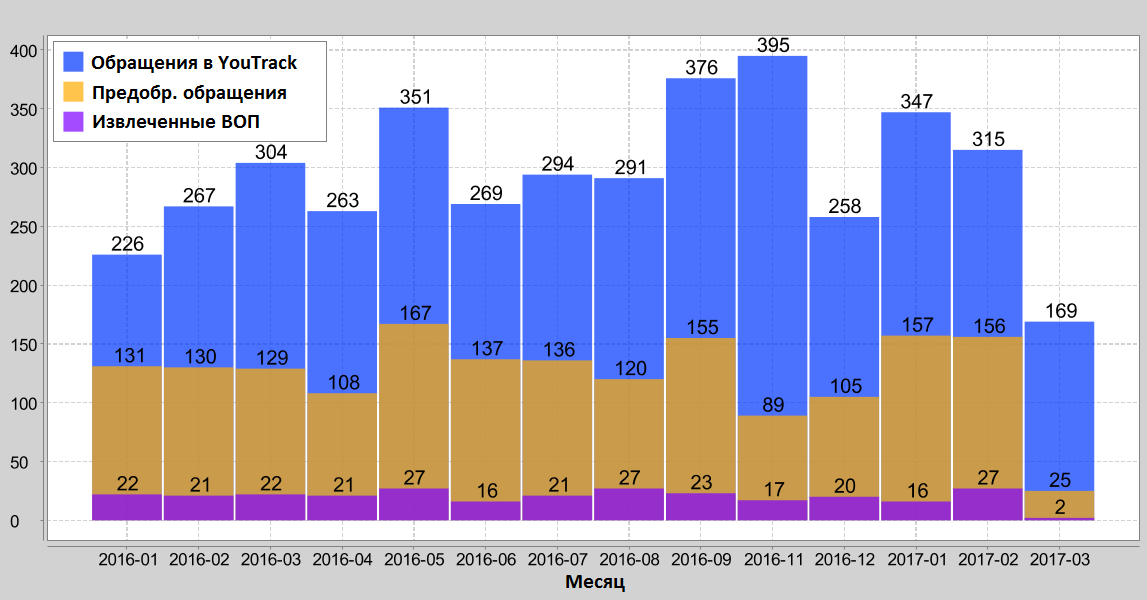
\includegraphics[width=11.5cm]{fig/tickets_distr.png}}
    \caption{Гистограмма извлеченных ВОП}
    \label{fig:tickets_distr}
\end{figure}

По графику видно, что медианное значение количества вопросов, на которое может быть расширен раздел с ЧЗВ, составляет 21 вопрос в месяц. В среднем доля ВОП составляет 6,8\%.

Как упоминалось ранее, анализируемые данные не являются предварительно размеченными, в связи с чем, отсутвует возможность посчитать полноту и точность решения. Воспользуемся другими способами оценки качества найденных ВОП, которые рассмотрены далее.

\section{Оценка влияния эвристик и параметров на качество ВОП}

Характеристики анализируемых данных включают:

\begin{itemize*}
\item 6500 обращений за период с января 2016 года по март 2017;
\item 19700 комментариев;
\item 45000 различных слов;
\item Тематическое модедлирование проводилось для 200 тем.
\end{itemize*}

В работе~\cite{original} установлено, что ВОП, признанные экспертами подходящими для публикации в ЧЗВ, имеют более высокие значения косинусного расстояния (\cite{original},~секция~VI--C). На основе этого для оценки качества разработанного способа извлечения ВОП воспользуемся следующими метрикиками: косинусное расстояние между вопросом и темой, косинусное расстояние между ответом и темой. Таблица~\ref{quality} показывает влияние этапов предобработки и параметров алгоритма на значения метрик. 

В первой строке показаны значения метрик для опимальных параметров алгоритма. Последующие строки описывают, какое изменение было внесено и как оно влияет на выбранные метрики качества по сравнению с оптимальными параметрами. Качество извлеченных ВОП считается тем выше, чем выше косинусное расстояние для вопроса и ответа.

По таблице~\ref{quality} видно, что применение эвристик предобработки и фильтров (за исключением фильтра тем) положительно влияет на косинус вопросов и ответов. Из чего можно сделать вывод о том, что применение соответсвубщих этапов ведет к повышению качества извлеченных ВОП. 

Помимо этого из таблицы~\ref{quality} можно сделать вывод о том, что изменение параметров в большую сторону позволяет находить меньшее количество более качественных, с точки зрения косинусного расстояния, ВОП. 

\begin{landscape}
\begin{table*}[t]
  \caption{Влияние эвристик и параметров на медианные значения метрик}
  \label{quality}
  \centering
  \begin{tabular}{|c|c|c||c|c|c|c|}
     \hline
      \parbox[t]{3cm}{\textbf{Исследуемый параметр}} &%
     \parbox[t]{2cm}{\textbf{Старое значение}} &%
     \parbox[t]{1.7cm}{\textbf{Новое значение}} &%
     \textbf{Перплексия} &%
     \parbox[t]{2cm}{\textbf{Количество ВОП}} &%
     \textbf{$\cos(Q,T)$} &%
     \textbf{$\cos(A,T)$} \\
	 \hline
     \parbox[t]{3cm}{Оптимальные\\параметры} &%
     - &%
     - &%
	 1864 &%
     357 &%
 	 0.396 &%
     0.413 \\
  	 \hline
     \parbox[t]{3cm}{Эвристики отображения (\ref{subsec:lnfheur})} &%
     вкл &%
     выкл &%
	 1971 &%
     361 &%
 	 0.371 &%
     0.395 \\
	 \hline
	 \parbox[t]{3cm}{Эвристики тем.\\модел. (\ref{subsec:ldaheur})} &%
     вкл &%
     выкл &%
	 2016 &%
     384 &%
 	 0.369 &%
     0.391 \\
	 \hline
\parbox[t]{3cm}{Фильтр\\обращений (\ref{subsec:ticketfilter})} &%
     вкл &%
     выкл &%
	 1924 &%
     403 &%
 	 0.370 &%
     0.388 \\
	 \hline
\parbox[t]{3cm}{Фильтр тем (\ref{subsec:topicfilter})} &%
     вкл &%
     выкл &%
	 1791 &%
     472 &%
 	 0.393 &%
     0.416 \\
     \hline
\parbox[t]{3cm}{Порог выбора\\темы LDA (\ref{subsec:lda})} &%
     0.25 &%
     0.0 &%
	 1853 &%
     376 &%
 	 0.366 &%
     0.404 \\
     \hline
\parbox[t]{3cm}{Порог выбора\\темы LDA (\ref{subsec:lda})} &%
     0.25 &%
     0.4 &%
	 1871 &%
     302 &%
 	 0.399 &%
     0.421 \\
     \hline
\parbox[t]{3cm}{Мин. значение\\косинуса (\ref{subsec:findqa})} &%
     0.15 &%
     0.0 &%
	 1860 &%
     394 &%
 	 0.337 &%
     0.359 \\
     \hline
\parbox[t]{3cm}{Мин. значение\\косинуса (\ref{subsec:findqa})} &%
     0.15 &%
     0.3 &%
	 1864 &%
     288 &%
 	 0.387 &%
     0.419 \\
     \hline         
\parbox[t]{3cm}{Мин. доля\\ВОП (\ref{subsec:deleteunfocusedtopics})} &%
     0.1 &%
     0.0 &%
	 1869 &%
     376 &%
 	 0.384 &%
     0.407 \\
     \hline
\parbox[t]{3cm}{Мин. доля\\ВОП (\ref{subsec:deleteunfocusedtopics})} &%
     0.1 &%
     0.2 &%
	 1850 &%
     324 &%
 	 0.391 &%
     0.417 \\
     \hline     
  \end{tabular}

\end{table*}
\end{landscape}

\section{Экспертная оценка}

Экспертная оценка проводилась только для оптимального набора параметров. Из данных, описанных в предыдущей секции, было извлечено 358 ВОП. Некоторые из характеристик полученных вопросно-ответных пар приведены в таблице~\ref{qainfo}.

\begin{table*}[tph!]
  \caption{Характеристики извлеченных ВОП}
  \label{qainfo}
  \centering
  \begin{tabular}{|L{4cm}|C{2cm}|}
     \hline
     \textbf{Количество ВОП} & 358\\%
	 \hline
	 \textbf{Ср. длина вопроса (симв.)} & 323\\%
	 \hline
     \textbf{$avg \cos(Q,T)$} & 0.401\\%
	 \hline
     \textbf{$avg \cos(A,T)$} & 0.412\\%
	 \hline
	 \textbf{Гармоническое ср.} & 0.406\\%
	 \hline
     \textbf{Ср. количество комментариев в исх. обращении} & 3.6\\
	 \hline
  \end{tabular}
\end{table*}

При проведении экспертного оценивания использовались индивидуальные оценки, основанные на мнениях независисмых друг от друга экспертов. Способ оценки~--- ранжирование. Ранжируемое свойство~--- корректность вопросно-ответной пары. Под корректностью ВОП подразумевается:

\begin{itemize*}
\item Пригодность вопроса для добавления в ЧЗВ;
\item Соответсвие ответа задаваемому вопроссу;
\item \quotes{Внешний вид} ВОП~--- наличие шумов (секция~\ref{sec:overview}), необходимость в редактировании.
\end{itemize*}

Экспертам было необходимо отнести каждый из оцениваемых ВОП к одной из следующих категорий:

\begin{enumerate*}
\item Подходит для публикации без редактирования;
\item Подходит для публикации с редактированием вопроса и/или ответа;
\item Не подходит для публикации. Некорректный вопрос;
\item Не подходит для публикации. Некорректный ответ;
\end{enumerate*}

Корректными считаются ВОП, относящие к категории 1 или 2.

В качестве экспертов выступили команда технической поддержки и команда технических писателей YouTrack~--- 4 человека. Для отображения ВОП и получения оценок использовался веб-интерфейс. Экспертам предлагалось последовательно оценивать по одной ВОП в случайном порядке. Экспертам были доступны только текст вопроса и ответа, дополнительные характеристики ВОП, как, например, косинусное расстояние между вопросом и темой, были скрыты. Ограничения на максимальное количество ВОП, оцениваемых одним экспертом установлено не было. Результаты представлены в таблице \ref{qualityExpert}.

\begin{table}[tph!]
\caption{Результаты экспертной оценки}
\label{qualityExpert}
\centering
\begin{tabular}{|c|c|c|}
\hline
Категория ВОП & Количество & Доля, \% \\
\hline
\parbox[t]{4cm}{\textbf{Общее количество}} & 358 & 100 \\

	 \hline
\parbox[t]{4cm}{1. Подходит для публикации без редактирования.} & 262 & 73 \\

	 \hline
\parbox[t]{4cm}{2. Подходит для публикации с редактированием вопроса и/или ответа.} & 17 & 5\\

	 \hline
\parbox[t]{4cm}{3. Не подходит для публикации. Некорректный вопрос.} & 17 & 5\\

	 \hline
\parbox[t]{4cm}{4. Не подходит для публикации. Некорректный ответ.} & 62 & 17\\
\hline
\end{tabular}
\end{table}

Доля подходящих для публикации ВОП составила 78\% (категории 1 и 2). В приложении~\ref{appx03} представлены примеры ВОП, принадлежащих к каждой из категорий.

\section{Резюме}

В данном разделе проведена оценка качества разработанной технологии извлечения ВОП. Определяется численная метрика качества ВОП: косинусное расстояние между вопросом и темой, косинусное расстояние между ответом и темой. 

Оценка влияния эвристик и параметров на качество ВОП показала, что используемые эвристики повышают качество извлекаемых ВОП. Повышение значений параметров алгоритма приводит к уменьшению количества извлекаемых ВОП, при жтом повышаются значения выбранных метрик качества.

Описана методика проведения экспертного оценивания. Вводится понятие корректных ВОП. По результатам экспертной оценки, проведенную работу можно считать успешной, поскольку:

\begin{itemize}
\item Достигнутый результат (78\%) превосходит резульататы работы~\cite{original} (37\%), использующей похожее решение;
\item Команда YouTrack удовлетворена достигнутыми результатами, планируется внедрение данного решения в рабочий процесс YouTrack.
\end{itemize}